% yaml_layers.tex
% Clean layered architecture diagram for Stata Journal
% Shows functional layers without exposing internal implementation details
% Author: João Pedro Azevedo
% Date: December 2025

\documentclass[tikz,border=10pt]{standalone}
\usepackage{tikz}
\usetikzlibrary{positioning, arrows.meta, fit, backgrounds}

\begin{document}

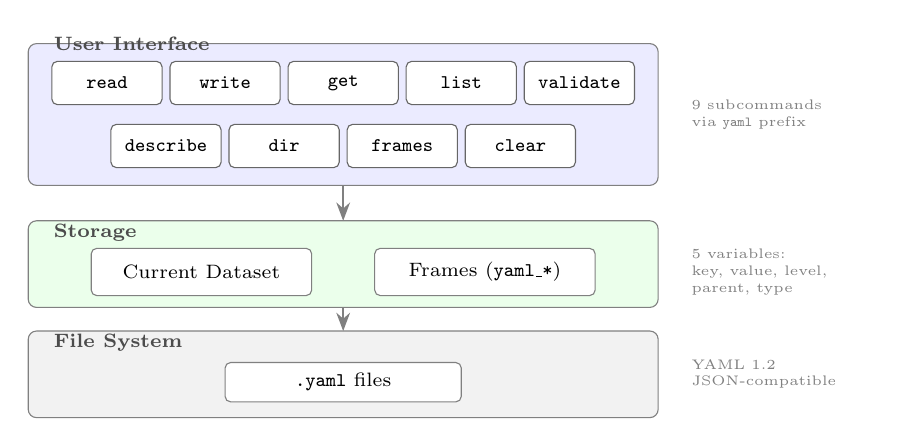
\begin{tikzpicture}[
    % Layer box style
    layer/.style={
        rectangle,
        rounded corners=3pt,
        draw=black!50,
        minimum width=8cm,
        minimum height=1.1cm,
        font=\small
    },
    % Command box style
    cmdbox/.style={
        rectangle,
        rounded corners=2pt,
        draw=black!60,
        fill=white,
        minimum width=1.4cm,
        minimum height=0.55cm,
        font=\scriptsize\ttfamily
    },
    % Arrow style
    arrow/.style={
        ->,
        >=Stealth,
        thick,
        black!50
    },
    % Label style
    lbl/.style={
        font=\scriptsize\bfseries,
        text=black!70
    }
]

% === Layer 1: User Interface ===
\node[layer, fill=blue!8, minimum height=1.8cm] (ui) at (0, 3.3) {};
\node[lbl, anchor=west] at (-3.8, 4.2) {User Interface};

% Subcommands in UI layer - first row
\node[cmdbox] at (-3, 3.7) {read};
\node[cmdbox] at (-1.5, 3.7) {write};
\node[cmdbox] at (0, 3.7) {get};
\node[cmdbox] at (1.5, 3.7) {list};
\node[cmdbox] at (3, 3.7) {validate};

% Second row of commands
\node[cmdbox] at (-2.25, 2.9) {describe};
\node[cmdbox] at (-0.75, 2.9) {dir};
\node[cmdbox] at (0.75, 2.9) {frames};
\node[cmdbox] at (2.25, 2.9) {clear};

% === Layer 2: Storage ===
\node[layer, fill=green!8] (storage) at (0, 1.4) {};
\node[lbl, anchor=west] at (-3.8, 1.8) {Storage};

\node[rectangle, draw=black!50, fill=white, rounded corners=2pt, 
      minimum width=2.8cm, minimum height=0.6cm, font=\scriptsize] 
      (dataset) at (-1.8, 1.3) {Current Dataset};
\node[rectangle, draw=black!50, fill=white, rounded corners=2pt,
      minimum width=2.8cm, minimum height=0.6cm, font=\scriptsize] 
      (frames) at (1.8, 1.3) {Frames (\texttt{yaml\_*})};

% === Layer 3: File System ===
\node[layer, fill=gray!10] (fs) at (0, 0) {};
\node[lbl, anchor=west] at (-3.8, 0.4) {File System};

\node[rectangle, draw=black!50, fill=white, rounded corners=2pt,
      minimum width=3cm, minimum height=0.5cm, font=\scriptsize] 
      at (0, -0.1) {\texttt{.yaml} files};

% === Arrows between layers ===
\draw[arrow] (0, 2.4) -- (0, 1.95);
\draw[arrow] (0, 0.85) -- (0, 0.55);

% === Side annotations ===
\node[font=\tiny, text=black!50, anchor=west, text width=2.2cm, align=left] 
    at (4.3, 3.3) {9 subcommands\\via \texttt{yaml} prefix};
\node[font=\tiny, text=black!50, anchor=west, text width=2.2cm, align=left] 
    at (4.3, 1.3) {5 variables:\\key, value, level,\\parent, type};
\node[font=\tiny, text=black!50, anchor=west, text width=2.2cm, align=left] 
    at (4.3, 0) {YAML 1.2\\JSON-compatible};

\end{tikzpicture}

\end{document}
